\chapter{SegRanks - Experiments With The Database of Annotations}

In this chapter we describe several experiments with the collected database of
annotations. 

\section{Overall Ranking of Annotated Systems}
\label{evaluating-annotated-systems}

In the first experiment we would like to show that the proposed method can be
used to produce overall ranking of the annotated systems which will be very
similar to the official human evaluation in WMT with much less human effort
\XXX{dolozit, pokud je to vubec pravda a pokud to vubec pujde}.

The obtained database contains a list of annotations for each extracted source
segment from each source sentence. A list can be empty (not all of the
sentences were annotated), it can contain more than one annotation (some
segments were annotated twice by an annotator, some segments were annotated by
multiple annotators), but most of the time it contains only one annotation.

An annotation is a mapping from the set of candidate segments to the set of
ranks ${1 \ldots N+1}$, where $N$ is the count of unique candidate segments.
(To discriminate the relative quality of all segments, annotators had available
$N$ ranks which could be all occupied when there are no ties. The rank $N+1$
represents the ``garbage'' category from the annotation application. However in
all of our experiments reported in this thesis we consider this category as one
more, the worst, rank). A Lower rank of a segment means that the candidate
segment was ranked better. This is an example \metoda{segment annotation} of a
source segment ``the huge volume'':

\begin{verbatim}
    {
      'velkému objemu' : 1,
      'obrovské hlasitosti' : 5,
      'obrovský objem' : 2,
      'obrovské množství' : 2,
    }
\end{verbatim}

We expanded these segment annotations with the information about the systems
which produced the segments. The ranks in the annotations are now indexed by
the system names.  If more systems translated a source segment as the same
candidate segment the candidate segment's rank is copied to all the systems.
This is the time when we use advantage of ranking short segments which are
often translated identically.  The following is the \metoda{system annotation}
after expansion of the above \metoda{segment annotation}:

\begin{verbatim}
    {
      'uedin-unconstrained' : 2,
      'commercial1' : 5,
      'commercial2' : 2,
      'CU-TectoMT' : 1,
      'onlineB' : 2,
      'onlineA': 2,
      'cu-funky' : 2,
      'cu-bojar' : 2,
      'uedin-wmt14': 2,
      'cu-depfix': 2
    }
\end{verbatim}

These rankings are now very similar to those obtained in the official WMT human
evaluation. These annotations are mostly interpreted as pairwise systems'
comparisons (for each combination of size 2 of all systems we have a pairwise
comparison), where the absolute values of the ranks and their absolute
differences between them are not considered. From above \metoda{system
annotation}, the following \metoda{pairwise comparisons} are be extracted (only
a few extracted pairwise comparisons are listed here for the sake of brevity,
generally $N \times (N-1) / 2$ pairwise comparisons are extracted, where $N$ is
number of all systems):

\begin{verbatim}
    [
      'uedin-unconstrained' < 'commercial1',
      'uedin-unconstrained' = 'commercial2',
      'uedin-unconstrained' > 'CU-TectoMT',
      ...
      'commercial1' > 'commercial2',
      'commercial1' > 'CU-TectoMT',
      ...
    ]
\end{verbatim}

The interpretation of these pairwise comparisons was changed several times
during the WMT workshops. Here, we use \metoda{Ratio of wins (ignoring ties)}
method, which was introduced by \perscite{bojar:grain:of:salt} and used in
WMT12 workshop \parcite{callisonburch:wmt12}. This method is based on a method
used in several WMT workshops before WMT12 and it is quite easy to compute and
interpret results.

For a given set $C$ of segment-level extracted pairwise comparisons
$(s_1,s_2,c)$, where 

\begin{equation*}
c = \begin{cases}
  win  & \text{if $rank(s_1) < rank(s_2)$} \\
  loss & \text{if $rank(s_1) > rank(s_2)$} \\
  tie  & \text{if $rank(s_1) = rank(s_2)$} \\
    \end{cases}
\end{equation*}

\noindent we define for each system $s$ the total number of wins, losses and ties:

\begin{equation*}
\begin{array}{rcl} 
  win(s)  & := & |\{(s,\bar{s},c) \in C; c = win\}| + |\{(\bar{s},s,c) \in C; c = loss\}| \\
  loss(s) & := & |\{(s,\bar{s},c) \in C; c = loss\}| + |\{(\bar{s},s,c) \in C; c = win\}| \\
  ties(s) & := & |\{(s,\bar{s},c) \in C; c = tie\}| + |\{(\bar{s},s,c) \in C; c = tie\}| \\
\end{array}
\end{equation*}

Then the \metoda{Ratio of wins (ignoring ties)} for a given system $s$ is
computed using the following formula:

\begin{equation*}
  E_{win}(s) = \frac{win(s)}{win(s) + loss(s)} 
\end{equation*}

\begin{table}
  \begin{center}
    \subfloat[Short segments judgements]{
      %\begin{center}
        \begin{tabular}{|l|c|}
          \hline
          \textbf{System} & \textbf{Score} \\
          \hline
           cu-depfix           &  0.5777 \\
           onlineB             &  0.5642 \\
           uedin-unconstrained &  0.5626 \\
           cu-bojar            &  0.5606 \\
           cu-funky            &  0.5566 \\
           uedin-wmt14         &  0.5498 \\
           onlineA             &  0.5007 \\
           CU-TectoMT          &  0.4485 \\
           commercial1         &  0.3992 \\
           commercial2         &  0.3492 \\
          \hline
        \end{tabular}
      %\end{center}
      \label{all-systems-segranks-results}
    }
    \subfloat[Official WMT14 judgements]{
      %\begin{center}
        \begin{tabular}{|l|c|}
          \hline
          \textbf{System} & \textbf{Score} \\
          \hline
          cu-depfix          &  0.6101 \\
          cu-bojar           &  0.6011 \\
          uedin-unconstrained&  0.5967 \\
          cu-funky           &  0.5823 \\
          onlineB            &  0.5439 \\
          uedin-wmt14        &  0.5285 \\
          onlineA            &  0.5039 \\
          CU-TectoMT         &  0.4473 \\
          commercial1        &  0.3617 \\
          commercial2        &  0.2780 \\
          \hline
        \end{tabular}
      \label{all-systems-wmt-results}
    }

  \end{center}

  \caption[Overall system rankings computed on short segment judgments]{Overall
    rankings of systems according to \metoda{Ratio of wins (ignoring ties)}
    score. You can see the results computed on both short segments judgements
    and on official WMT14 human judgements side by side to compare the
  differences.}

  \label{all-systems-results}
\end{table}

\subsection{Results}

The overall ranking of systems, which participated in WMT14 Translation Task in
English-Czech direction, according to the \metoda{Ratio of wins (ignoring
ties)} computed on the short segments judgements is reported in the table
\ref{all-systems-segranks-results}.

To compare our method with the classic method of judging whole sentences, we
have also computed the \metoda{Ratio of wins (ignoring ties)} on the judgements
collected during WMT14 manual evaluation. You can see these results in the
table \ref{all-systems-wmt-results}.

You can notice that the range of scores computed on the short segments
judgements is much narrower (0.35 --- 0.58) than the range of scores computed
on the sentence judgements (0.28 --- 0.61). This can be explained by the
following: If system A beats system B in a sentence-level judgement of a
particular sentence it does not necessarily mean that in segment-level judging
system A will be better than system B on all segments of the sentence. System A
will be probably better on a majority of the segments (but even that does not
have to be always true). When computing the ratio of wins on the sentence-level
judgements, system A gets one win and system B gets one loss. However, when
computing the ratio of wins on the segment-level system A gets for example two
wins and one loss, system B one win and two losses. It should be clear now that
computing expected wins on the sentence-level judgements is coarser while our
method is more fine-grained.  \XXX{Co z toho vlastne plyne? Je to dobre, nebo
spatne?}

The overall rankings of systems obtained by both of the methods is very
similar. However, there are two changes when comparing to the sentence-level
judgments results: system online-B is better and system cu-bojar is worser
according to the segments-level judgments results. We try to explain this in the Analysis.

\subsection{Analysis}

To see the difference between the segment-level judgements and sentence-level
judgements we have computed Kendall tau rank correlation coefficient, also
known as Kendall's $\tau$, between segment-level pairwise comparisons and
sentence-level pairwise comparisons. This coefficient is used to measures how
often a set of pairwise rankings agrees with another set of pairwise rankings.
The basic formula for Kendall's $\tau$ is:

\begin{equation*}
  \tau = \frac{|Concordant| - |Discordant|}{|Concordant| + |Discordant|}
\end{equation*}

\noindent where $Concordant$ is the set of pairwise combination where both sets
of pairwise rankings agrees with each other and $Discordant$ is the set of
pairwise combination where the sets do not agree in pairwise ranking.
\XXX{mozna vyhodit predchozi vetu}  We will discuss the Kendall's $\tau$ in
more details in chapter \ref{metrics}. Here we computed $|Concordant|$ as the
number of pairwise segment-level judgments which agrees with the corresponding
sentence-level judgment. Similarly, $|Discordant|$ is the number of those which
does not agree with the corresponding sentence-level judgment. In this section
we does not consider any tied pairwise comparisons.

\begin{table}
  \begin{center}
    \subfloat[Better systems]{
      %\begin{center}
        \begin{tabular}{|l|c|}
          \hline
          \textbf{System}                   &   $\tau$ \\
        \hline
         cu-funky            &        0.428 \\
         cu-depfix           &        0.405 \\
         onlineB             &        0.398 \\
         cu-bojar            &        0.394 \\
         uedin-uncon. &        0.390 \\
         uedin-wmt14         &        0.363 \\
         onlineA             &        0.312 \\
         CU-TectoMT          &        0.270 \\
         commercial1         &        0.166 \\
         commercial2         &        0.123 \\
          \hline
        \end{tabular}
      %\end{center}
      \label{sentence-segments-judgments-correlations-better}
    }
    \,
    \subfloat[Worse systems]{
      %\begin{center}
        \begin{tabular}{|l|c|}
          \hline
          \textbf{System}                   &   $\tau$ \\
       \hline
         commercial2         &        0.492 \\
         commercial1         &        0.441 \\
         CU-TectoMT          &        0.385 \\
         onlineA             &        0.328 \\
         uedin-uncon. &        0.260 \\
         uedin-wmt14         &        0.257 \\
         cu-funky            &        0.230 \\
         cu-bojar            &        0.227 \\
         cu-depfix           &        0.225 \\
         onlineB             &        0.225 \\
          \hline
        \end{tabular}
      \label{sentence-segments-judgments-correlations-worse}
    }
    \,
    \subfloat[All systems]{
      %\begin{center}
        \begin{tabular}{|l|c|}
          \hline
          \textbf{System}                   &   $\tau$ \\
        \hline
         commercial2         &        0.394 \\
         cu-funky            &        0.348 \\
         commercial1         &        0.345 \\
         uedin-uncon. &        0.341 \\
         cu-depfix           &        0.335 \\
         CU-TectoMT          &        0.333 \\
         cu-bojar            &        0.328 \\
         onlineB             &        0.321 \\
         onlineA             &        0.320 \\
         uedin-wmt14         &        0.317 \\
          \hline
        \end{tabular}
      \label{sentence-segments-judgments-correlations-all}
    }

  \end{center}

  \caption[Correlations between the segment-level judgments and sentence-level
  judgments]{Kendall's $\tau$ correlations between the segment-level and
    sentence-level judgments. For a given system we computed the correlation on
    all pairwise comparisons including the given system. The table
    \ref{sentence-segments-judgments-correlations-better} contains correlations
    computed on sentence-level judgments where the given system was better, the
    table \ref{sentence-segments-judgments-correlations-worse} is computed on
    sentence-level comparisons where the given system was worse and finally the
    table \ref{sentence-segments-judgments-correlations-all} was computed on
    all pairwise comparisons including the system. The systems are sorted by
    the correlation in reverse order.} 

  \label{sentence-segments-judgments-correlations}
\end{table}

The computed correlations are tabulated in the table
\ref{sentence-segments-judgments-correlations}. The order of the systems in the
table \ref{sentence-segments-judgments-correlations-better} is quite similar to
the order of systems in the overall rankings (table \ref{all-systems-results});
better systems have higher correlation than worse systems.  This is somehow
expected: Better systems, which were more often ranked better in the
sentence-level judgements are also more likely to be ranked better in the
segment-level judgments.  You can also read the table in the following way: If
a sentence of system cu-funky was ranked better on sentence-level it is very
likely (71\%) that the segments of the sentence were ranked better also. On the
other hand, if system commercial2 was ranked better on sentence-level only a
little more than half of the segments were ranked better also. The table
\ref{sentence-segments-judgments-correlations-worse} is similar but in reversed
order.

The influence of a system's quality should be canceled out in the table
\ref{sentence-segments-judgments-correlations-all}. You can see, that systems
cu-bojar and onlineB have the Kendall's $\tau$ lower (although not the lowest).
This together with the fact that both systems lies in a cluster of systems of
very similar quality is consistent with their change in the overall ranking of
systems. This, however, does not explain that.

For the explanation of the differences between the overall rankings computed on
sentence-level and segment-level judgments we have to look into the data. We
want to find candidate translations for which the sentence judgments disagree as
much as possible with the segment judgments. To quantify this property we have
defined \metoda{disagreement quotient}:

\begin{equation*}
  q_d(s,n) = \frac{
    win_{seg}(s,n) / (win_{seg}(s,n) + loss_{seg}(s,n))
  }{
    win_{sent}(s,n)/(win_{sent}(s,n) + loss_{sent}(s,n))
  }
\end{equation*}

\noindent where $s$ is a system, $n$ is a sentence number, $win_{seg}(s,n)$ is
the number of segment-level comparisons where the $n$-th candidate sentence
translated by system $s$ won and $loss_{sent}(s,n)$ is the number of
comparisons in which the candidate sentence losses. Finally, $win_{sent}(s,n)$
and $loss_{sent}(s,n)$ are defined similarly for the sentence-level
comparisons.

Using this measure we have found candidate sentence translations which were
ranked high by segment-level judgments but ranked low by the sentence-level
judgments.  We have listed candidate sentences with the highest
\metoda{disagreement quotient} and tried to analyze the cause of the
disagreement between the sentence-level and segment-level judgments. In the
following we present a few of these sentences with comments. The extracted
segments which were ranked are in bold.

\begin{center}
  \begin{tabular}{rp{11cm}}

    \textbf{Source:} & Airlines began charging for \textbf{the first and second
  checked bags} in 2008. \\

    \textbf{Candidate:} & Letecké linky začaly nabíjení pro \textbf{první a
  druhý odbavených zavazadel} v roce 2008.
  
  (Sentence 715, online-B) \\

  \end{tabular}
\end{center}

\noindent The translation of the segment is relatively good, the case of the
noun phrase is wrong but the meaning could be understood. The reason why the
whole sentence was ranked poorly is probably the word ``nabíjení'' (``Charging
a battery'' in English), which is obviously a wrong lexical choice of the MT
system. Unfortunately this word is not covered by the only ranked segment. A
similar problem is also in the following sentence:

\begin{center}
  \begin{tabular}{rp{11cm}}

    \textbf{Source:} & I want to fulfil \textbf{my role of dad and husband}. \\

    \textbf{Candidate:} & Chci, aby splnil \textbf{svou roli táty a manžela}.
    
    (Sentence 559, cu-bojar) \\

  \end{tabular}
\end{center}

\noindent The translation of the segment is perfect but the subject of the
candidate translation is wrongly expressed as a third person. The whole
sentence is therefore correctly ranked as a poor translation. And again this is
not covered by the extracted segments.

\begin{center}
  \begin{tabular}{rp{11cm}}

    \textbf{Source:} & \textbf{Samsung, Huawei and HTC} all manufacture phones
    that operate on \textbf{Google's Android operating system}, which competes
    fiercely \textbf{with Apple and Microsoft mobile products}. \\

    \textbf{Candidate:} & \textbf{Samsung, Huawei a HTC} všechny výrobní
    telefony, které pracují \textbf{android operační systém Google}, který
    konkuruje \textbf{zuřivě a Applu Microsoftu mobilním produktům}.
    
    (Sentence 484, CU-TectoMT) \\

  \end{tabular}
\end{center}

The problem here is again in the predicate. The verb ``manufacture'' is wrongly
translated as the adjective ``výrobní'' (``manufactured'' in English).

In all the previous examples, a predicate was wrongly translated but
unfortunately it was not covered in the extracted segments and therefore
reflected in segment-level judgments. This seems to be the main disadvantage of
this method, extracted segments sometimes do not cover predicates which are
very important for annotator when judging quality of machine translation.

We have also listed candidate translations with the lowest \metoda{disagreement
quotient} (a candidate was highly ranked by sentence-level judgments but lowly
ranked by system-level judgments). However, these candidates were not so
interesting and we cannot see any general pattern there. We feel that the
sentences which are ranked much better in segment-level judgments than in
sentence-level judgments are much more serious problem.

\section{Evaluating New Systems}
\label{evaluating-new-systems}

Machine translation systems often translate a short source segment identically.
This was one of our main motivation for ranking translations of short segments.
As you saw in the previous chapter, evaluating the annotated systems using the
short segments annotations works even it has some shortcomings.  It would be
very useful if we could use the database of annotations to evaluate also yet
unseen systems. The more annotated systems we have in the database the more
likely it is that an unseen MT system produce a translation of a short segment
which is already in the database. We will call this situation a \metoda{hit},
if the translated segment is not already annotated, we will call it a
\metoda{miss}.

Because we didn't have any spare systems which were not annotated, we did the
following trick: in each step we choose one system and removed its segments
from the database of annotations. Then we consider this system as unseen and
tried to match the system's segments with the segments left in the database. We
call this trick \metoda{leave-one-out}.

\begin{table}
  %\begin{center}
  \centering
    \subfloat[uedin-uncnstr., hits: 0.67]{
        \begin{tabular}{|l|c|}
          \hline
           system                   &   score \\
          \hline
           uedin-uncnstr. &   0.633 \\
           cu-depfix           &   0.580 \\
           uedin-wmt14         &   0.576 \\
           onlineB                &   0.571 \\
           cu-bojar            &   0.564 \\
           cu-funky            &   0.560 \\
           onlineA                &   0.499 \\
           CU-TectoMT          &   0.425 \\
           commercial1         &   0.377 \\
           commercial2         &   0.329 \\
          \hline
         \end{tabular}
      \label{}
    }
    \,
    \subfloat[commercial1, hits: 0.28]{
        \begin{tabular}{|l|c|}
          \hline
           system                   &   score \\
          \hline
           commercial1         &   0.581 \\
           uedin-uncnstr. &   0.557 \\
           onlineB                &   0.552 \\
           uedin-wmt14         &   0.540 \\
           cu-depfix           &   0.535 \\
           cu-funky            &   0.525 \\
           cu-bojar            &   0.523 \\
           onlineA                &   0.472 \\
           CU-TectoMT          &   0.422 \\
           commercial2         &   0.346 \\
          \hline
         \end{tabular}
      \label{}
    }
    \,
    \subfloat[commercial2, hits: 0.28]{
        \begin{tabular}{|l|c|}
          \hline
           system                   &   score \\
          \hline
           commercial2         &   0.570 \\
           onlineB                &   0.552 \\
           uedin-uncnstr. &   0.548 \\
           cu-depfix           &   0.535 \\
           cu-bojar            &   0.529 \\
           cu-funky            &   0.524 \\
           uedin-wmt14         &   0.523 \\
           onlineA                &   0.457 \\
           CU-TectoMT          &   0.423 \\
           commercial1         &   0.386 \\
          \hline
         \end{tabular}
      \label{}
    }
    
    \subfloat[CU-TectoMT, hits: 0.45]{
        \begin{tabular}{|l|c|}
          \hline
           system                   &   score \\
          \hline
           CU-TectoMT          &   0.649 \\
           cu-depfix           &   0.600 \\
           cu-bojar            &   0.584 \\
           cu-funky            &   0.575 \\
           onlineB                &   0.528 \\
           uedin-uncnstr. &   0.522 \\
           uedin-wmt14         &   0.502 \\
           onlineA                &   0.450 \\
           commercial1         &   0.373 \\
           commercial2         &   0.339 \\

          \hline
         \end{tabular}
      \label{}
    }
    \,
    \subfloat[onlineB, hits: 0.52]{
        \begin{tabular}{|l|c|}
          \hline
           system                   &   score \\
          \hline
           onlineB                &   0.689 \\
           uedin-uncnstr. &   0.584 \\
           cu-depfix           &   0.578 \\
           cu-funky            &   0.567 \\
           cu-bojar            &   0.567 \\
           uedin-wmt14         &   0.564 \\
           onlineA                &   0.511 \\
           CU-TectoMT          &   0.406 \\
           commercial1         &   0.360 \\
           commercial2         &   0.320 \\
          \hline
         \end{tabular}
      \label{}
    }
    \,
    \subfloat[onlineA, hits: 0.47]{
        \begin{tabular}{|l|c|}
          \hline
           system                   &   score \\
          \hline
           onlineA                &   0.649 \\
           onlineB                &   0.584 \\
           uedin-uncnstr. &   0.577 \\
           uedin-wmt14         &   0.568 \\
           cu-depfix           &   0.566 \\
           cu-bojar            &   0.555 \\
           cu-funky            &   0.546 \\
           CU-TectoMT          &   0.411 \\
           commercial1         &   0.365 \\
           commercial2         &   0.318 \\
          \hline
         \end{tabular}
      \label{}
    }
    
    \subfloat[cu-funky, hits: 0.74]{
        \begin{tabular}{|l|c|}
          \hline
           system                   &   score \\
          \hline
           cu-funky            &   0.630 \\
           cu-depfix           &   0.600 \\
           cu-bojar            &   0.582 \\
           uedin-uncnstr. &   0.559 \\
           onlineB                &   0.557 \\
           uedin-wmt14         &   0.542 \\
           onlineA                &   0.491 \\
           CU-TectoMT          &   0.446 \\
           commercial1         &   0.378 \\
           commercial2         &   0.331 \\
          \hline
         \end{tabular}
      \label{}
    }
    \,
    \subfloat[cu-bojar, hits: 0.88]{
        \begin{tabular}{|l|c|}
          \hline
           system                   &   score \\
          \hline
           cu-bojar            &   0.588 \\
           cu-depfix           &   0.582 \\
           cu-funky            &   0.564 \\
           onlineB                &   0.562 \\
           uedin-uncnstr. &   0.559 \\
           uedin-wmt14         &   0.545 \\
           onlineA                &   0.498 \\
           CU-TectoMT          &   0.449 \\
           commercial1         &   0.392 \\
           commercial2         &   0.346 \\
          \hline
         \end{tabular}
      \label{}
    }
    \,
    \subfloat[cu-depfix, hits: 0.93]{
        \begin{tabular}{|l|c|}
          \hline
           system                   &   score \\
          \hline
           cu-depfix           &   0.587 \\
           cu-bojar            &   0.570 \\
           cu-funky            &   0.566 \\
           onlineB                &   0.562 \\
           uedin-uncnstr. &   0.561 \\
           uedin-wmt14         &   0.548 \\
           onlineA                &   0.498 \\
           CU-TectoMT          &   0.449 \\
           commercial1         &   0.394 \\
           commercial2         &   0.345 \\
          \hline
         \end{tabular}
      \label{}
    }

    \caption[Results of evaluating unseen systems by exact matching]{The
      results of evaluating unseen systems using the exact matching and the
      \metoda{leave-one-out} trick. Each subtable is marked by the leaved
      system.  You can also see the hit rates. The table for system uedin-wmt14
      is omitted for the sake of brevity.}

  \label{one-out-results}
\end{table}

\subsection{Exact Matching of candidate segments}
\label{exact:matching}

The most obvious way to evaluate an unseen translation is to compute the
\metoda{Ratio of wins (ignoring ties)} of all the systems (including the unseen
one) only on the hit segments. We extracted the pairwise comparisons from all
the segment annotations where the segment of the unseen system was hit and
computed the \metoda{Ratio of wins (ignoring ties)} only on that extracted
comparisons. We performed this experiment for all the systems using the
\metoda{leave-one-out} trick.

You can see the results of this experiment in the table \ref{one-out-results}.
We also report \metoda{hit} rate, which is the ratio of hits to all (miss +
hits).

The average hit rate is 58.8 \% which is above our expectation. However, as you
can see, the hit rate varies a lot across the leaved out systems. This is
caused by the fact, that some systems are very similar, they use the same tools
and/or training data. For example all the systems cu-bojar, cu-depfix, cu-funky
are based on the Moses SMT toolkit and their hit rates are very high (0.74 ---
0.93).

As you can see the obtained orderings of the systems are not very good. The
winning system in each of the tables is that which was leaved out. Which is
obviously wrong. Besides that, systems similar to the leaved out system in each
system gets also much better rank. For example, when the leaved system is one
of the systems cu-bojar, cu-depfix and cu-funky, the other two of this group
are right bellow the leaved out system. This could be explained by the
following statement: MT systems are more likely to agree on a good translation
of a segment than on a bad translation.

To support this statement we have performed an analysis of some sentences from
the test set. In the following examples of sentences, we have marked the hit
segments by \hit{green} and the missed segments by \miss{red}:


\begin{center}
  \begin{tabular}{rp{11cm}}

    \textbf{Source:} &

    So, \hit{still no Words} With Friends, the \miss{online Scrabble-type game}
    that \hit{actor Alec Baldwin} was playing \hit{on his smartphone in 2011}
    \miss{when he was famously} booted off \miss{an American Airlines jet} for
    refusing to turn off the device while the plane \hit{was parked at the
    gate}.

    
    \\

    \textbf{Candidate:} &
    
    Takže \hit{stále žádná slova} s přáteli, \miss{online hra Scrabble typ} že
    \hit{herec Alec Baldwin} si hrál \hit{na jeho smartphone v roce 2011},
    \miss{kdy mu byl slavně} spuštěn z \miss{American Airlines jet} za odmítnutí
    vypněte zařízení, zatímco letadlo \hit{bylo zaparkováno u brány}.
    
    (Sentence 2976, onlineA) \\

  \end{tabular}
\end{center}

\noindent You can see that the green hits are translated relatively correctly
and are understandable. We cannot say the same about the missed segments.

\begin{center}
  \begin{tabular}{rp{11cm}}

    \textbf{Source:} &

    \miss{Amongst other things}, it showed that the Americans even monitored
    \hit{the mobile phone} \miss{of German Chancellor Angela Merkel}.
    
    \\

    \textbf{Candidate:} &

    \miss{Kromě jiných věcí} ukázalo, že Američané i sledovali \hit{mobilní
    telefon} \miss{Germana kancléře Angely Merkelové}.

    (Sentence 2945, CU-TectoMT) \\

  \end{tabular}
\end{center}

\noindent The missed segment ``Kromě jiných věcí'' in this sentence is
traslated quite well (so the above statement does not hold here). However, the
only hit segment here ``mobilní telefon'' is translated correctly and the
missed segment ``Germana kancléře Angely Merkelové'' is not translated
correctly. Judging how easy is a segment to translate is even more difficult
than judging the translations, but you may agree with us that the hit segment
``the mobile phone'' is easy to translate and the missed segment ``of German
Chancellor Angela Merkel'' is much more difficult to translate. We can see this
also in the last example:


\begin{center}
  \begin{tabular}{rp{11cm}}

    \textbf{Source:} &

    They had \miss{searched frantically for their missing dog} and posted
    appeals \hit{on social networking sites} after she had ran \hit{into the
    quarry} \miss{following the minor accident}.
    
    \\

    \textbf{Candidate:} &

    Měli zoufale \miss{hledal své chybějící psa} a odvolání \hit{na sociálních
    sítích} poté, co se dostal \hit{do lomu} \miss{po drobné nehody}.
    
    (Sentence 77, uedin-wmt14) \\

  \end{tabular}
\end{center}

\noindent Both of the hit segments are translated very well and we can say that
they are also very easy to translate. On the other hand, the missed segments
are understandable but not perfect. Compared to the green segment, they are
also more difficult to translate.

Following the manual analysis we can conclude that MT systems are really more
likely to agree on the better translations. This however prevent us to match
the segments exactly, because it gives us very overestimated scores for the
unseen candidates.

\subsection{Matching the Closest Segment by Edit Distance}
\label{match:editdistance}

We would like to compute the scores on all the annotated segments to avoid the
problem from the previous subsection. A natural way to approximate the
``correct'' ranks of unseen segments is to use the rank of the segment from the
database with the closest edit distance. We use the character based Levenshtein
distance which is defined as the minimum number of insertion, deletion and
substitution of characters required to transform a given string to another:

\begin{equation*}
  lev(a,b) = \#insertions + \#delition + \#substitution
\end{equation*}

\noindent If more segments in the database has the minimal distance to the ``unseen'' 
segment, we pick one of them randomly.


\begin{table}
  %\begin{center}
    \centering

\subfloat[uedin-uncnstr., AED: 2.0]{
\begin{tabular}{|l|c|}
\hline
 system                   &   score \\
\hline
 uedin-uncnstr. &   0.598 \\
 cu-depfix           &   0.575 \\
 onlineB                &   0.562 \\
 cu-bojar            &   0.558 \\
 cu-funky            &   0.554 \\
 uedin-wmt14         &   0.548 \\
 onlineA                &   0.498 \\
 CU-TectoMT          &   0.446 \\
 commercial1         &   0.396 \\
 commercial2         &   0.346 \\
\hline
\end{tabular}
}
\,
\subfloat[commercial1, AED: 5.4]{
\begin{tabular}{|l|c|}
\hline
 system                   &   score \\
\hline
 cu-depfix           &   0.564 \\
 onlineB                &   0.552 \\
 uedin-uncnstr. &   0.550 \\
 cu-bojar            &   0.547 \\
 cu-funky            &   0.544 \\
 uedin-wmt14         &   0.537 \\
 commercial1         &   0.502 \\
 onlineA                &   0.487 \\
 CU-TectoMT          &   0.435 \\
 commercial2         &   0.333 \\
\hline
\end{tabular}
}
\,
\subfloat[commercial2, AED: 5.7]{
\begin{tabular}{|l|c|}
\hline
 system                   &   score \\
\hline
 cu-depfix           &   0.558 \\
 onlineB                &   0.548 \\
 uedin-uncnstr. &   0.545 \\
 cu-bojar            &   0.540 \\
 cu-funky            &   0.538 \\
 uedin-wmt14         &   0.532 \\
 commercial2         &   0.489 \\
 onlineA                &   0.483 \\
 CU-TectoMT          &   0.429 \\
 commercial1         &   0.379 \\
\hline
\end{tabular}
}

\subfloat[CU-TectoMT, AED: 3.9]{
\begin{tabular}{|l|c|}
\hline
 system                   &   score \\
\hline
 cu-depfix           &   0.565 \\
 CU-TectoMT          &   0.563 \\
 onlineB                &   0.553 \\
 uedin-uncnstr. &   0.551 \\
 cu-bojar            &   0.548 \\
 cu-funky            &   0.544 \\
 uedin-wmt14         &   0.539 \\
 onlineA                &   0.488 \\
 commercial1         &   0.387 \\
 commercial2         &   0.337 \\
\hline
\end{tabular}
}
\,
\subfloat[onlineB, AED: 3.1]{
\begin{tabular}{|l|c|}
\hline
 system                   &   score \\
\hline
 onlineB                &   0.621 \\
 cu-depfix           &   0.573 \\
 uedin-uncnstr. &   0.559 \\
 cu-bojar            &   0.556 \\
 cu-funky            &   0.552 \\
 uedin-wmt14         &   0.546 \\
 onlineA                &   0.496 \\
 CU-TectoMT          &   0.443 \\
 commercial1         &   0.395 \\
 commercial2         &   0.344 \\
\hline
\end{tabular}
}
\,
\subfloat[onlineA, AED: 3.4]{
\begin{tabular}{|l|c|}
\hline
 system                   &   score \\
\hline
 onlineA                &   0.588 \\
 cu-depfix           &   0.570 \\
 onlineB                &   0.556 \\
 uedin-uncnstr. &   0.554 \\
 cu-bojar            &   0.552 \\
 cu-funky            &   0.549 \\
 uedin-wmt14         &   0.541 \\
 CU-TectoMT          &   0.440 \\
 commercial1         &   0.391 \\
 commercial2         &   0.341 \\
\hline
\end{tabular}
}

\subfloat[cu-funky, AED: 1.7]{
\begin{tabular}{|l|c|}
\hline
 system                   &   score \\
\hline
 cu-funky            &   0.600 \\
 cu-depfix           &   0.574 \\
 onlineB                &   0.561 \\
 uedin-uncnstr. &   0.559 \\
 cu-bojar            &   0.557 \\
 uedin-wmt14         &   0.546 \\
 onlineA                &   0.496 \\
 CU-TectoMT          &   0.445 \\
 commercial1         &   0.396 \\
 commercial2         &   0.346 \\
\hline
\end{tabular}
}
\,
\subfloat[cu-bojar, AED: 0.4]{
\begin{tabular}{|l|c|}
\hline
 system                   &   score \\
\hline
 cu-bojar            &   0.580 \\
 cu-depfix           &   0.576 \\
 onlineB                &   0.562 \\
 uedin-uncnstr. &   0.561 \\
 cu-funky            &   0.555 \\
 uedin-wmt14         &   0.548 \\
 onlineA                &   0.499 \\
 CU-TectoMT          &   0.447 \\
 commercial1         &   0.398 \\
 commercial2         &   0.348 \\
\hline
\end{tabular}
}
\,
\subfloat[cu-depfix, AED: 0.2]{
\begin{tabular}{|l|c|}
\hline
 system                   &   score \\
\hline
 cu-depfix           &   0.579 \\
 onlineB                &   0.564 \\
 uedin-uncnstr. &   0.563 \\
 cu-bojar            &   0.561 \\
 cu-funky            &   0.556 \\
 uedin-wmt14         &   0.550 \\
 onlineA                &   0.501 \\
 CU-TectoMT          &   0.448 \\
 commercial1         &   0.399 \\
 commercial2         &   0.349 \\
\hline
\end{tabular}
}

\caption[Results of evaluating unseen systems by edit distance matching]{The results of
  evaluating unseen systems using the edit distance matching and
  \metoda{leave-one-out} trick. Each subtable is marked by the leaved system.
  The abbreviation AED stands for average edit distance which is computed
across all segments . The table for system uedin-wmt14 is omitted for the sake
of brevity.}

  \label{edit-distance-results}
\end{table}

Similarly to the previous experiment we extracted the pairwise comparisons and
computed the \metoda{Ratio of wins (ignoring ties)}. You can see the results
tabulated in the table \ref{edit-distance-results}. For each leaved out system,
we also report the average edit distance (AED) of the unseen segments to the closest
segments in the database.

The overall rankings of the systems are much more reasonable compared to the
exact matching, although they are still not perfect. The scores of systems
which were leaved out are not always the best in the obtained rankings but they
are still heavily overestimated. This shows not only that systems are more
likely to agree on the better translations than on the worse ones, but also
that they produce translations which are closer to better translations than to
other translations of similar quality. Our notion of that idea is that a good
translation is a point  in a high-dimensional space and candidate translations
are points around the good translation. Now let's have a few points around the
good translation representing the translations in the database. When we get a
new point it is quite likely in this high-dimensional space that the closest
point is the good translation. You can see an illustration of this situation in
two dimensions in the figure \ref{translation-space-illustration}. \XXX{Neni to
uz moc velke fantazirovani?} If we do not have enough candidates in the
database it is quite likely that for a given unseen candidate the closest
candidate is the good translation and not any other candidate translation of
similar quality. \XXX{V tomto odstavce zamenit good translation za better
translation, zmenit obrazek?}

\begin{figure}
    \begin{center}
        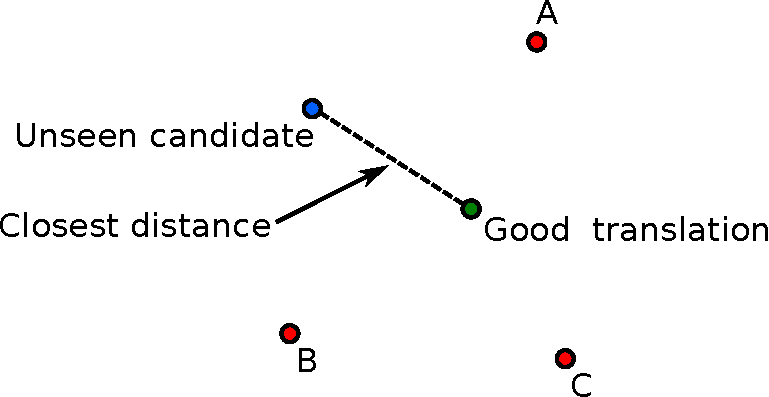
\includegraphics[width=8cm]{img/translation-space.pdf}
    \end{center}

    \caption[An illustration of a space of translations]{An example of a good
    translation with only a few candidate translations around it. If a number
  of dimensions is higher than the number of candidates it is intuitively quite
probable that the closest point to a new unseen candidate is the good
translation.}
    \label{translation-space-illustration}
\end{figure}

The average edit distances vary a lot. Systems cu-bojar, cu-depfix and cu-funky
have very low AED (0.2 --- 1.7), because they are very similar to each other.
Systems CU-TectoMT, onlineA and onlineB are in the middle of the AED range (3.1
--- 3.9) and since they are quite solitary in the set of ranked systems we can
consider their AEDs as representative values.  Systems commercial1 and
commercial2 have the highest AEDs. This could be explained by the fact that
both of the systems are rule based and produce dissimilar translations to those
generated by the statistical based systems. It is, however, interesting that
their translations are not even similar to each other. You can see the distribution of the absolute
counts with respect to the edit distance plotted in the figure
\ref{absolute-counts-per-distance}.

\begin{figure}
    \begin{center}
        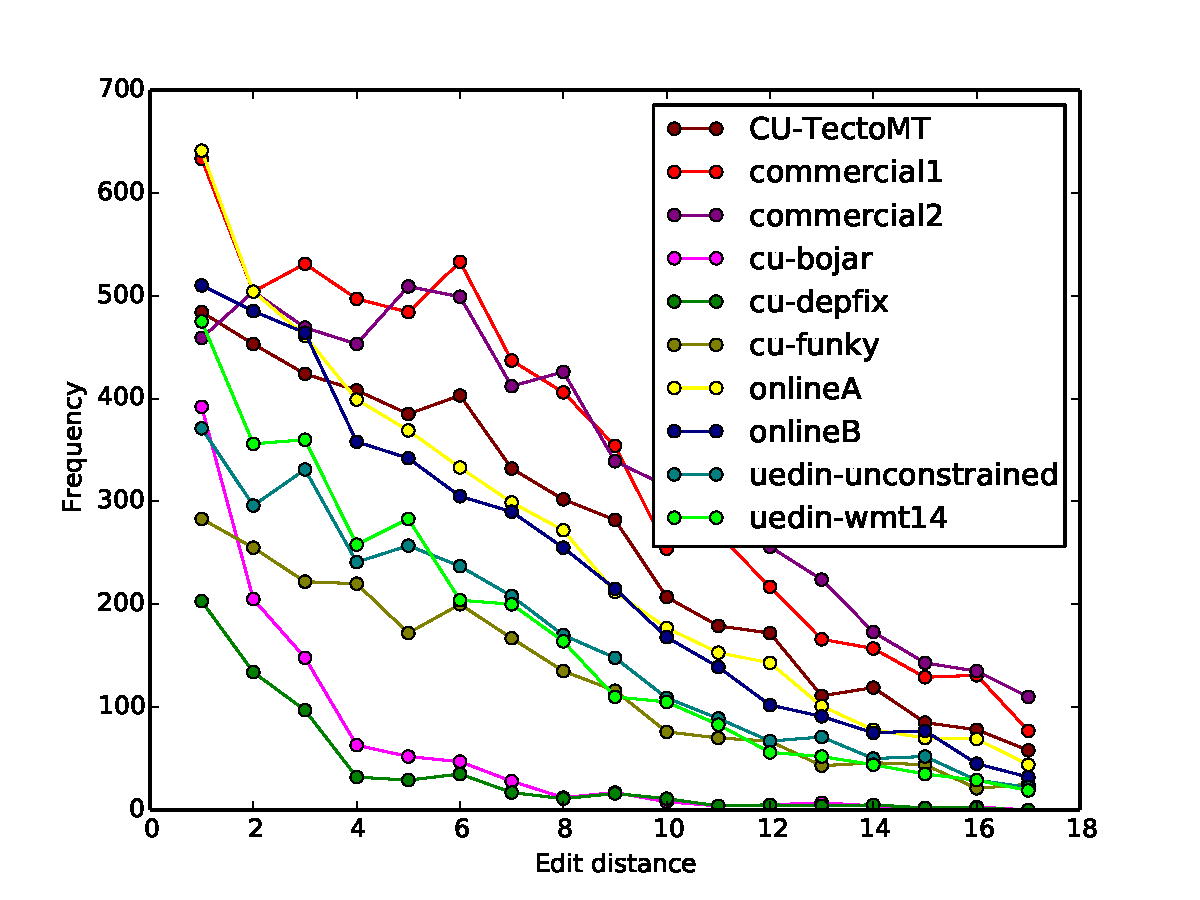
\includegraphics[width=14cm]{img/absolute-counts-per-distance.pdf}
    \end{center}

    \caption[Absolute counts of matched segments with respect to the edit distance]
    {Absolute counts of segments with respect to the edit distance}

    \label{absolute-counts-per-distance}
\end{figure}


To support the above statement (that the closest segment to an unseen candidate
is more likely to be of better quality) we have performed the following
analysis: For each leaved out system we computed how often the closest segment
has better, equal or worse rank than the ``unseen'' segment (We can actually do
that, because we know the true rank of the segment removed from the database).
We computed these relative frequencies only on the missed segments (the closest
segment was not the same segment). You can see this analysis performed for the
individual systems in the table \ref{edit-distance-matching-analysis}.  You can
also see how these relative frequencies change with with a change of the edit
distance in the figure \ref{better-worse-equal-with-edit-distance}. More than a
half of the closest segments has better rank than the original segments and
only 20.6 \% of the segments have the same rank. This is really very poor
because it means that our approximation method which ranks unseen translations
has the accuracy only 20.6 \%. This accuracy does not differ much for
individual systems but there is an expected trend of similar systems (cu-bojar,
cu-depfix) having this accuracy slightly higher. 

As you can see in the figure \ref{better-worse-equal-with-edit-distance} the
relative number of closest systems which are ranked better grows quite
significantly with the edit distance. The relative number of the worse segments
is quite stable (around 0.3) and does not change significantly with the edit
distance. The relative number of closest segments which are equally raked as
the source segment is decreasing with the edit distance. For example, for the
segments whose edit distance to the closest segment is 17, only 10 percent of
the closest segments is equally ranked, which is really poor. 


\begin{table}
  \centering
\begin{tabular}{|lrrr|}
  \hline
  \textbf{Unseen system}            &   \textbf{Worse} &   \textbf{Equal} &   \textbf{Better} \\
  \hline
   commercial1         &   27.9 \% &   19.0 \% &    53.1 \% \\
   commercial2         &   23.3 \% &   17.5 \% &    59.2 \% \\
   cu-bojar            &   22.5 \% &   31.5 \% &    46.0 \% \\
   cu-depfix           &   32.7 \% &   33.2 \% &    34.0 \% \\
   cu-funky            &   28.8 \% &   23.8 \% &    47.4 \% \\
   CU-TectoMT          &   25.8 \% &   18.6 \% &    55.6 \% \\
   onlineA             &   28.1 \% &   20.4 \% &    51.5 \% \\
   onlineB             &   33.3 \% &   20.9 \% &    45.8 \% \\
   uedin-unconstrained &   32.4 \% &   22.3 \% &    45.3 \% \\
   uedin-wmt14         &   31.6 \% &   23.4 \% &    45.1 \% \\
  \hline
   All               &   28.1 \% &   20.6 \% &    51.2 \% \\
  \hline
\end{tabular}

\caption[Comparisons of unseen and the closest systems]{Comparisons of unseen
and the closest system. This table shows how often the closest segment in the
database was worse, equally good or better than the original ``unseen''
segment. These relative frequencies were computed only on missed segments
(which weren't already in the database).}

  \label{edit-distance-matching-analysis}
\end{table}

\begin{figure}
    \begin{center}
        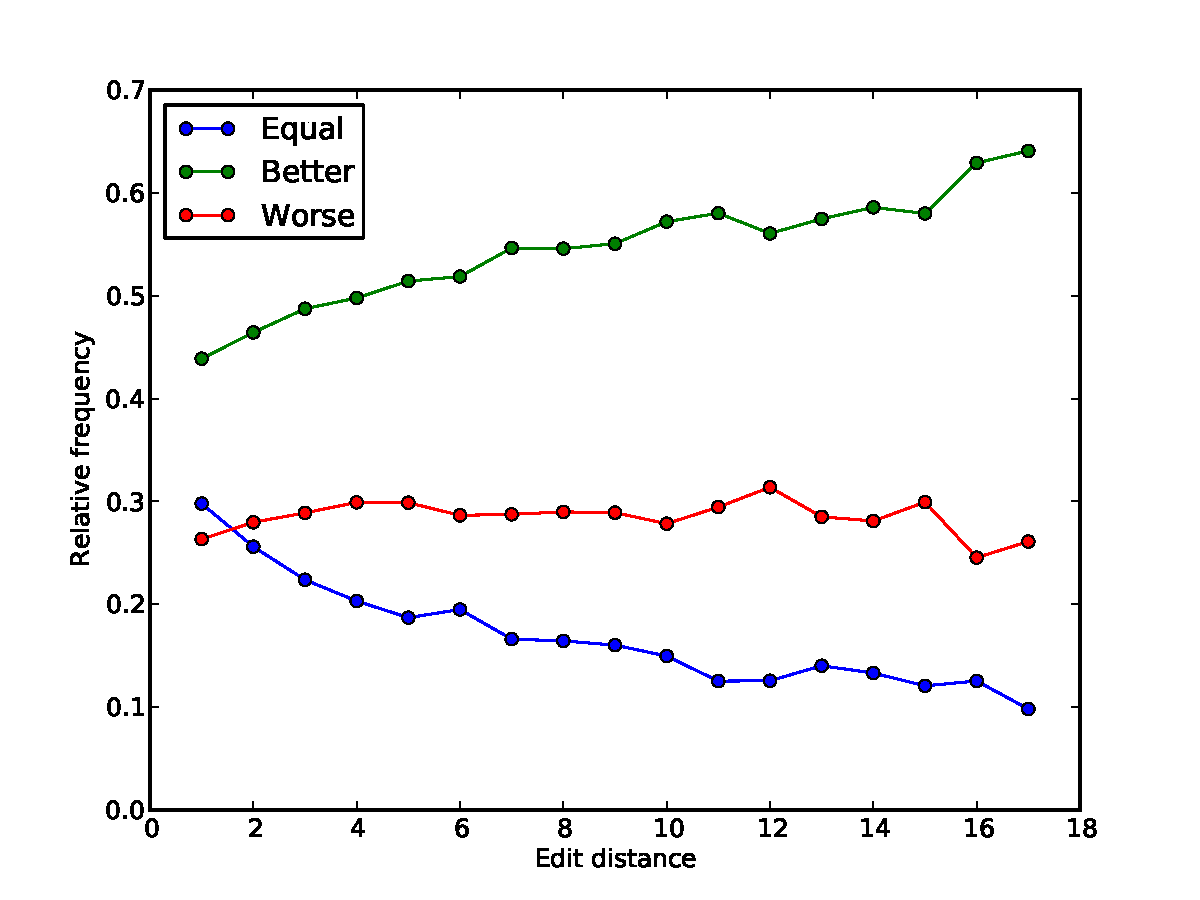
\includegraphics[width=14cm]{img/per-distance.pdf}
    \end{center}

    \caption[Comparisons of unseen and the closest systems with respect to the
    edit distance]{Comparisons of unseen and the closest systems with respect
    to the edit distance. The results in this figure are computed on all the
systems.}

    \label{better-worse-equal-with-edit-distance}
\end{figure}




We also listed a few example candidate segments in the table
\ref{segments-closest} together with the corresponding closest segments from
the database and their distances. We also report whether the closest segment
was ranked better, equal or worse than the ``unseen'' one.

\begin{table}
  \begin{center}
    \begin{tabular}{|p{5.5cm}p{5.5cm}rc|}
      \hline
      \textbf{Unseen segment} & \textbf{Closest segment} & \textbf{D} & \textbf{C} \\
      \hline
      s dokumenty upřednostňujícím doprovodem hradu & se dokumenty favorizovat doprovod hradu & 18 & \worse{} \\ \hline
      ze 120 domova m2 & z 120 m2 domova & 7 & \better{} \\ \hline
      vaše ústa ohřívá protein & vaše ústa zahřívání bílkovin & 10 & \better{} \\ \hline
      videokonference & videokonferenci & 1 & \better{} \\ \hline
      popřel užívání kokainu a & popřela užívání kokainu a & 1 & \worse{} \\ \hline
      přibližně šedesát- drah kilometru & přibližně šedesát-dráha kilometru & 3 & \equal{} \\ \hline
      v Liverpoolském porotním soudu & Liverpool Korunního soudu & 11 & \better{} \\ \hline
      je nesmysl v gravitaci filmu & Je nesmysl ve filmu gravitace & 15 & \better{} \\ \hline
      Pak 64,23 \% oprávněných voličů & pak 64,23 \% oprávněných voličů & 1 & \better{} \\ \hline
      podle DPA agentury & podle DPA agentury té & 3 & \worse{} \\ \hline
    \end{tabular}
  \end{center}

  \caption[Example candidates and the closest segments]{ Example candidates and
    the closest segments. The last but one column (\textbf{D}) stands for
    distance and contains distances of the unseen candidates to the closest
    segments. The last column (\textbf{C}) stands for comparison; the closest
  segment is either worse (\worse{}), equally good (\equal{}) or better
(\better{}) than the original unseen segment.}

  \label{segments-closest}
\end{table}

We have to unfortunately conclude, that the proposed method, which reuses the
database for evaluating unseen translations, does not work. We analyzed the
results and the main cause of this failure seems to be that the systems tend to
agree on better translations and their translations tend to be more similar to
better translations in the database so we cannot predict their rank accurately. 

\subsection{Enhancing reference translation with good candidates from the database}
\label{enhancing:bleu}

Following the conclusions from the previous two subsections, it seems that
errors in machine translation are very unique. Any database of bad examples
(bad translations) is therefore very sparse. It is very well known fact that a
number of correct translations is very high \parcite{bojar2013scratching}. It
seems, however, that the number of bad translations is much higher and
therefore it make more sense to use a database of good translations. 

In the following experiment we therefore use only the good candidate segments
from the annotated database. The approach used here is, however, different from
the previous experiments. We would like to measure how similar are candidates
to the good translations from the database. This is very similar to what
automatic metrics do when measuring similarity between a candidate and a
reference translations. We have therefore decided to use one of the standard
metrics -- \metric{BLEU} -- to measure this similarity. First, we are going to
introduce the metric and then we are going to customize it for our experiment. 

\begin{table}
  \begin{center}
      \subfloat[\metric{SegRanksBLEU}, correlation: 0.9745 ]{
        \begin{tabular}{|l|c|}
          \hline
          \textbf{System} & \textbf{Score} \\
          \hline
          cu-depfix & 0.305 \\
          cu-funky & 0.302 \\
          uedin-unconstrained & 0.302 \\
          cu-bojar & 0.300 \\
          uedin-wmt14 & 0.296 \\
          onlineB & 0.289 \\
          onlineA & 0.259 \\
          CU-TectoMT & 0.225 \\
          commercial1 & 0.176 \\
          commercial2 & 0.160 \\
          \hline
        \end{tabular}
      \label{enhanced-bleu-results}
    }
    \,
    \subfloat[\metric{BLEU}, correlation: 0.9751]{
        \begin{tabular}{|l|c|}
          \hline
          \textbf{System} & \textbf{Score} \\
          \hline
          cu-depfix & 0.221 \\
          cu-bojar & 0.221 \\
          cu-funky & 0.221 \\
          uedin-unconstrained & 0.220 \\
          uedin-wmt14 & 0.215 \\
          onlineB & 0.207 \\
          onlineA & 0.187 \\
          CU-TectoMT & 0.157 \\
          commercial1 & 0.114 \\
          commercial2 & 0.102 \\

          \hline
        \end{tabular}
      \label{bleu-results}
    }

  \end{center}

  \caption[Overall system ranking according to \metric{SegRanksBLEU} and
  \metric{BLEU} scores]{Overall system ranking according to
  \metric{SegRanksBLEU} and \metric{BLEU} scores. Please see the chapter
  \ref{metrics} for the details of computation of the reported correlations.}

  \label{segranksbleu:experiment}
\end{table}

Metric \metric{BLEU} was developed by \perscite{Papineni02bleu:a} and it is the
most used metric in the machine translation evaluation. It is defined as the
geometric mean of n-gram precisions for $n \in \{1 \ldots N\}$, where $N$ is
usually 4. More precisely, for a candidate $c$ and reference translations $r_i$
where $i \in I$, let the clipped count of an n-gram $g$ be defined as follows:

\begin{equation*}
    \text{count}_{clip}(g,c,r) = \min \left( \cnt(g, c), ~ \max_{i \in I} \left( \cnt(g, r_i) \right) \right)
\end{equation*}

\noindent where $\cnt(g, s)$ denotes the count of n-gram $g$ in the sentence
$s$. The modified precision $p_n$ is then defined as:

\begin{equation*}
    p_n = \frac{
        \sum_{g \in \text{n-grams}(c)} \text{count}_{clip}(g,c,r)
    }{
        \sum_{g \in \text{n-grams}(c)} \cnt(g,c)
    }
\end{equation*}

\noindent Using the computed n-gram precisions, we can compute the final
\metric{BLEU} score:

\begin{equation*}
        BLEU = BP \cdot \exp \left( \frac{1}{N} \sum_{i = 1}^N \log p_n \right) 
\end{equation*}

\noindent where $BP$ is the brevity penalty (meant to penalize short outputs to
discourage improving precision at the expense of recall) defined as follows:

\begin{equation*}
    BP = \left\{ 
  \begin{array}{l l}
    1 & \quad \text{if } |c| > |r|\\
    \exp(1-|r|/|c|) & \quad \text{if } |c| \leq |r| \\
    \end{array} \right.
\end{equation*}

\noindent where $|c|$ and $|r|$ are the lengths of the candidate and reference
translations respectively. In the case of multiple reference translations,
$|r|$ could be the average length, the maximum length or the length closest to
the candidate $c$.

This experiment consists of two steps. In the first step we select good segment
translations from the short segments database. In the second step we use the
selected good segment translations to enhance reference translations when
computing \metric{BLEU}.

Since the assigned ranks in the database are relative, we cannot know which
segments are really good in the term of the absolute quality. We have to assume
that there is at least one good candidate translation among the ranked
candidates and consider all candidate segments with the best rank as the good
translations. We select these candidate segments for each source segment for
each sentence.

Finally, we use the selected good segments as the reference translations in
addition to the original reference sentence translated by human expert.  Since
the new references are only short segments and do not cover a whole sentence,
we use only the length of the original reference sentence in the computation of
the brevity penalty. To distinguish this method from the standard \metric{BLEU}
with the single official reference translation, we will call this method
\metric{SegRanksBLEU}.

Please note, that introducing the new reference
translations, which do not change the brevity penalty, can only increase the
clipped counts of n-grams occurring in the short segments.  Candidates will be
rewarded for having n-grams which are also in the good segment translations in
the database.

You can see the overall rankings of the evaluated systems as given by
\metric{SegRanksBLEU} and \metric{BLEU} in the table
\ref{segranksbleu:experiment}. As expected, the \metric{SegRanksBLEU} scores
are really much higher than \metric{BLEU}. However, the reported system level
correlations of these two metrics are almost equal (correlation of
\metric{SegRanksBLEU} is even a little bit lower).  \XXX{Jak tohle zanalyzovat
a vysvetlit?}


\section{Tuning Systems}
\label{tuning-systems}

Automatic metrics are not used only for evaluating already developed systems on
test sets. They are also often used when tuning a system to choose the
parameters of a model which gives the best metric score computed on a
development test set. One of the methods utilizing automatic metrics for system
tuning is Minimum Error Rate Training (MERT). We will describe the theory
behind the MERT in the following subsection a then we will experiment with
using the short segments rank database in the MERT.

\subsection{Minimum Error Rate Training}

Most of the statistical machine translation systems model the posterior
probability of producing a sentence translation $e$ given a source sentence $f$
using a log-linear model \parcite{Och:2002}: 

\newcommand{\vect}[1]{\boldsymbol{#1}}
\begin{equation}
    P(e \mid f) = %p_{\lambda_1^M} (e \mid f) =
    \frac
        {\exp \left(\sum_{m=1}^M \lambda_m h_m(e,f) \right)}
        {\sum_{e'} \exp \left(\sum_{m=1}^M \lambda_m h_m(e',f)\right)}
    = \frac
    {\exp \left( \vect{\lambda} \cdot \vect{h}(e,f)  \right)}
    {\sum_{e'} \exp \left(\vect{\lambda} \cdot \vect{h}(e',f)\right)}
\end{equation}

\noindent where the vector $\vect{h}(e,f) = \{ h_1(e,f), h_2(e,f), \ldots ,
h_M(e,f) \}$ is a feature vector and the vector $\vect{\lambda} = \{\lambda_1,
\lambda_2, \ldots, \lambda_M \}$ is a feature weight vector. It can be easily
shown that when searching for the best candidate $e_{best}$, the above
log-linear formula could be simplified to the following:

\begin{equation}
  e_{best}  =  \argmax_e \left\{ P(e \mid f) \right\}
  =  \argmax_e \left\{ \vect{\lambda} \cdot \vect{h}(e,f) \right\}
\end{equation}

Now the problem with this log-linear model is how to find the weight vector
$\vect{\lambda}$ which would give the best translations. And this is what the
MERT method solves.

Let $F = \{f_i;~ i \in I\}$ be a held out corpus in the source language and $R
= \{r_i;~ i \in I\}$ be a corresponding reference translation. Traditionally
the best weight vector $\vect{\lambda}$ can be found using the maximum
likelihood principle:

\begin{equation}
  \vect{\hat\lambda} = \argmax_{\vect{\lambda}} \left\{ \prod_{i \in I}
  P_{\vect{\lambda}} (e_i \mid f_i ) 
\right\}
\end{equation}

\noindent This optimization problem has some very nice properties: there is
one global optimum and there are algorithms which converge to this optimum.
\perscite{Och:2003}, however, argues that that there is no proof that this
method gives the best weights with respect to the translation quality. 

He suggested to choose the weight vector $\vect{\lambda}$ which produces the
best translation of the heldout data. We can measure the quality of the
translation using an automatic metric $m(E,R)$, where $E$ is the set of
candidate translations produced by the MT system and $R$ is a set of reference
translation. We are therefore going to minimize the score (or minimize it in
the case the metric is error based and returns lower scores for better
translations) of the metric:

\begin{equation}
  \vect{\hat\lambda} = \argmax_{\vect{\lambda}} \left\{ m( \hat{E}(F,
  \vect{\lambda}), R ) \right\}
    \label{eq:errorrate-opt}
\end{equation}

\noindent where $\hat{E}(F, \vect{\lambda})$ is the corpus $F$ translated with
the weights $\vect{\lambda}$ and $\hat{e}(f, \vect{\lambda})$ is the
translation of a sentence $f$ with weights $\vect{\lambda}$:

\begin{equation}
  \hat{E}(F, \vect{\lambda}) = \left\{ \hat{e}(f_i, \vect{\lambda});~i \in I\right\}
    \label{eq:corpus-translation}
\end{equation}

\begin{equation}
  \hat{e}(f, \vect{\lambda}) = 
    \argmax_{e} \left\{ \vect{\lambda} \cdot \vect{h}(e, f) \right\}
    \label{eq:sentence-translation}
\end{equation}

The criterion \eqref{eq:errorrate-opt} is, however, not so easy to optimize. It
contains argmax operation and therefore it is not smooth and it is not possible
to use a gradient based method. It has also a lot of local maximums.
\perscite{Och:2003} therefore suggested to use Powell's algorithm
\parcite{Powell:1964} which does not need gradient to optimize a function.

In each step, Powell's algorithm starts at a point from which it goes in
several directions (possibly also in random directions) and optimizes the
function along the lines which originate at the start point using a given line
optimization method. The most optimal point found on the lines is then used as
the new starting point in the next step. 

The Powell's algorithm depends on an efficient line optimization method. Och
proposed a method which takes advantage of log-linear model properties. In the
following we limit the space of the optimization problem to a line defined by
the following equation:

\begin{equation}
  \vect{\lambda}(\gamma) = \vect{\lambda'} + \gamma \vect{d}
  \label{eq:line}
\end{equation}

\noindent where $\vect{\lambda'}$ defines a starting point and the vector
$\vect{d}$ defines a direction of the line. Now, we can reformulate the limited
optimization problem:

\begin{equation}
  \hat{\gamma} = \argmax_{\gamma \in \mathbb{R}} \left\{ m(\hat{E}(F,\vect{\lambda}(\gamma)),R) \right\}
    \label{eq:line-opt}
\end{equation}

When we apply the line equation \ref{eq:line} in the argmax operator which
choose the best translation in the equation \ref{eq:sentence-translation}, we
get the following.

\begin{eqnarray}
  \hat{e}(f, \vect{\lambda}(\gamma))
    & = & \argmax_{e} \left\{ \vect{\lambda}(\gamma) \cdot  \vect{h}(e, f) \right\} \\
    & = & \argmax_{e} \left\{ \vect{\lambda'} \cdot \vect{h}(e, f) + \gamma \vect{d} \cdot \vect{h}(e, f) \right\} \\
    & = & \argmax_{e} \left\{ t(e,f) + \gamma \cdot m(e,f) \right\} \label{eq:argmax}
\end{eqnarray}

\noindent where the scalars $t(e,f)$ and $m(e,f)$ are constant for a given
candidate $e$. This means, that each candidate $e$ specifies a line given by
the equation $x = t(e,f) + \gamma \cdot m(e,f)$ which computes the candidate
score for the parameter $\gamma$. The argmax operator in the equation
\eqref{eq:argmax} then choose the candidate whose line is the highest in a
given $\gamma$. You can see this situation illustrated in the figure
\ref{fig:lines}.  The line optimization method finds all the intersections of
the lines where the best candidate (with the highest model score) changes. The
intersections found for each sentence in the heldout data are then merged to
obtain intervals of $\gamma$ in which the $\gamma$ does not change the set of
the highest score candidates.  For each interval, the metric score is computed
and the optimal $\gamma$ is chosen from the interval with the highest metric
score. Since the metrics are often computed from sentence decomposable
statistics, we can easily update the metric's score in each interval boundary
by subtracting the old sentence's statistics and adding the new sentence's
statistics.

\begin{figure}
    \begin{center}
        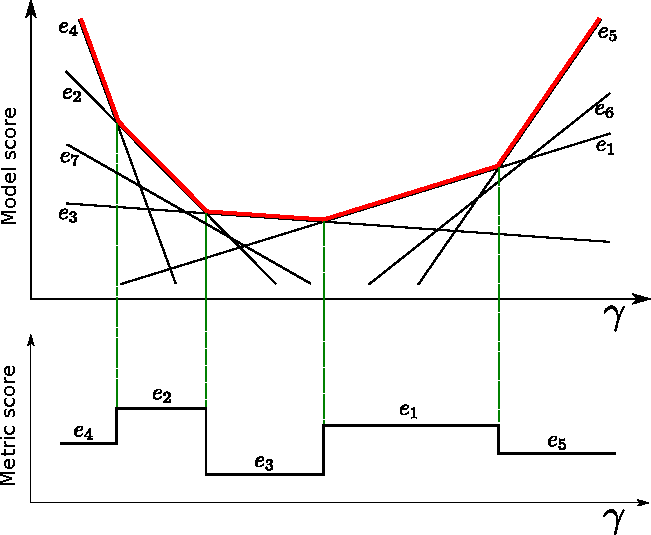
\includegraphics[width=10cm]{img/mert.pdf}
    \end{center}

    \caption[An illustration of the line optimization in MERT]{
      An illustration of the line optimization in MERT. You can see two sentences and their
      candidate translations represented by the lines. The best candidate in each interval
      is marked by the red line. The bottom part of the figure illustrates how the metric score
      depends on $\gamma$.
}

    \label{fig:lines}
\end{figure}

The last difficulty in the MERT method is that we cannot easily enumerate all
the candidate sentences. For that reason the n-best list approximation is used:
the decoder produce $n$ best translations for each sentence and only these $n$
translations are considered during the optimization. A problem arise when the
optimal weight vector found during the optimization gets too far from the
weight vector used to produce the initial n-best list. For that reason a new
n-best list is produced with the new weights, it is merged with previous n-best
lists and optimization process is run again in new MERT iteration. When the
optimal weight vector converges or a maximum number of iterations is reached
the MERT method ends. 

\subsection{Experiments with MERT}

MERT method is most often used with BLEU metric even it does not have the best
correlation with human judgments (see the chapter \ref{metrics} for more
details). However, there is a lot of experiments with utilizing also other
automatic metrics in recent time. In WMT11 \parcite{wmt11}, there was a shared
task in which participants tuned a common system with different metrics. The
tuned systems were then evaluated by humans and some of them outperformed the
baseline system tuned with BLEU.

It is not feasible to employ any sort of human evaluation directly in the MERT
process. On the one hand human evaluation is very slow and expensive, on the
other hand MERT requires to evaluate very long n-best list in each iteration.
There are some suggestions to do the manual evaluation in a clever way and
lower the amount of manual work. For example \perscite{human-in-the-loop}
noticed that a lot of short segments is repeated in a n-best list and therefore
suggest to extract these short segments from a n-best list in each MERT
iteration and let humans rank them. (Actually our short segment extraction
method was partially inspired by this work). However they did not try this
method in an actual MERT run yet for lack of resources. 

We believe that a much less expensive way to introduce an element of human
evaluation in MERT method is to use some sort of semi-automatic metric in which
a certain amount of manual work is needed at the beginning and then the metric
evaluates translations automatically. In this subsection, we therefore
experiment with previously introduced metrics which rely on the collected
database of short segment ranks.

\subsubsection{Tuned System}

The system we tried to tune is the system cu-bojar \parcite{tamchyna2014},
which we also used previous sections as one of the evaluated systems. This
system is Moses-based and combines several different approaches:

\begin{itemize}
  \item factored phrase-based Moses model
  \item domain-adapted language model
  \item deep-syntactic MT system TectoMT
\end{itemize}

The parallel data used to train the phrase tables consists of 14.83 million
parallel sentences taken from the CzEng corpus \parcite{bojar:czeng} and 0.65
millions of sentences taken from the Europarl corpus \parcite{koehn:europarl}.
The monolingual data used to train language models consists of 215.93 million
sentences taken from the Czech side of the CzEng corpus and from 5 sources of
news domain. 

They used their baseline systems to translate WMT test sets from years
2012--2014.  These translation were then used to retrieve similar Czech
sentences using information retrieval techniques which were then used to train
the domain-adapted language model.

The deep-syntactic MT system TectoMT was used to translate WMT test sets from
years 2007--2014. These new synthetic parallel training data were then used to 
train an additional phrase table. 

Please note that both the domain-adapted language model and the TectoMT phrase
table were also trained on the data we use as development set and test set so
that tuning can assign appropriate weights to them.

There is 15 component weights to tune in total. \perscite{tamchyna2014} of
course tuned their system cu-bojar when participating in the translation shared
task but we use their system before it was tuned by them to tune it ourselves. 

We used the implementation of MERT which is distributed with Moses
toolkit\footnote{\url{http://www.statmt.org/moses/}}. It is implemented in C++
and new metrics are created by subclassing the base \pojem{Scorer} class. Since
the annotated database is stored in Python data structures and since a
development in Python is much easier and faster, we have implemented new
\pojem{PythonScorer} which is an universal wrapper around an arbitrary Python
scorer class, implemented using the Python C API.


\subsubsection{Metric Variants}

Our original idea was that we will use the alignment produced by the Moses
decoder during translating the n-best list to project the extracted short
source segments to the target side to have candidates which would be extracted
the same way as the ranked segments in the database. Unfortunately the
alignment produced by Moses decoder is very sparse and unreliable (which may be
caused by a bug in the code) so we had to get along without the alignment.

The naive approximation is to just test whether the ranked candidate segments
from the database also occurs in evaluated sentences. The first metric we use
in MERT experiment is therefore very similar to the \metoda{Exact Matching}
method in the section \ref{exact:matching}. For each ranked source segment we
test if any of its candidate segment occurs in the evaluated sentence. If it
does we extract all pairwise comparisons inferred from the matched segment. If
more candidate segments occurs in the evaluated translation, we choose the
longest segment (assuming that the sorter segments are just substring of the
longest one). The final score is then computed as \metoda{Ratio of wins
(ignoring ties)}. We call this metric \metric{ExactMatch} in the following.

Even if the hit rate (percentage of segment candidates which are already ranked
in the database) computed on a whole n-best list would be 100 \%, the
\metric{ExactMatch} metric still does not evaluate whole sentences and could be
too coarse and harsh. Moreover, if the hit rate drops during the tuning, the
metric score would be computed on a very small percentage of development set
and would be very unstable. To ensure the tuning is stable, we interpolate all
the metrics in this section (if not said otherwise) together with BLEU with
equal weights. We also tried to tune using the \metric{ExactMatch} metric
solely but the tuned system translated very badly and the hit rate dropped very
low during the tuning. We could explain this by that the system was tuned to
translate a few ranked segments well (so these segments were hits) but other
segments were missed and translated badly. The optimal metric score was
therefore computed on a very small fraction of the development set and did not
reflect the overall quality of the translation.

Since we do not have the alignment and cannot extract the candidate segments
exactly, we unfortunately cannot use the method introduced in the subsection
\ref{match:editdistance} which matches the closest segment in the database by
edit distance.  To avoid the shortcomings of the \metric{ExactMatch} metric
(the metric is not computed on all the extracted source segments and an unseen
system is more likely to cause hit in the database with better translations) we
propose another variant called \metric{PenalizeUnknown}. This variant differs
to \metric{ExactMatch} in that it considers all missed segments as the worst
translations. We agree that the assumption that all unseen and unranked
segments are wrong is not correct, but this approach could increase the hit
rate. The question is then, whether we prefer to have a system which produces a
lot of segments which were already ranked (even badly) or a system which
produces a lot of unranked segments which we hope to be of better quality.

The last variant we experiment with is \metric{SegRanksBLEU} metric introduced
in subsection \ref{enhancing:bleu}. Because this metric is already based on
BLEU metric (and use the reference translation) we do not interpolate it with
BLEU anymore.


\subsubsection{Results and Analysis}

You can see the results of the tuned system in the table \ref{mert:results}. We
used the tuned systems to translate the test set (newstest2013) and then we
evaluated these translations automatically and manually. For the automatic
evaluation we used metrics \metric{BLEU} \parcite{Papineni02bleu:a} and
\metric{CDER} \parcite{Leusch06cder:efficient}. We have also conducted a small
scale manual evaluation. For each evaluated system, we randomly sampled
\XXX{100} sentences which were translated differently by the baseline and by
the evaluated system. \XXX{Two} annotators then compared the sampled
sentences with the corresponding translations produced by the baseline system.
Their task was to choose which sentence is better or whether they are of the
same quality. We report how many of the sampled sentences were better and
better-or-equal than the corresponding baseline translation.


\begin{table}
  \centering
  \begin{tabular}{|r|c|cc|cc|}
    \hline
    & \textbf{\#Mert} & \multicolumn{2}{|c|}{\textbf{Automatic}} & \multicolumn{2}{|c|}{\textbf{Manual}} \\
    & \textbf{iter-} & \multicolumn{2}{|c|}{\textbf{Evaluation}} & \multicolumn{2}{|c|}{\textbf{Evaluation}} \\
    \textbf{Tunable metric} & \textbf{ations} & \textbf{BLEU} & \textbf{CDER}  & $>$ & $\ge$ \\
    \hline
    \metric{BLEU} (baseline) & 11 & 0.1782 & 0.3855 & --- & --- \\
    \metric{ExactMatch}      & 20 & 0.1637 & 0.3674 & \XXX{} & \XXX{} \\
    \metric{PenalizeUnknown} &  8 & 0.1772 & 0.3850 & \XXX{} & \XXX{} \\
    \metric{SegRanksBLEU}    &  & \XXX{} & \XXX{} & \XXX{} & \XXX{} \\
    \hline
  \end{tabular}

  \caption[Results of systems tuned on SegRanks based metrics]{Results of
    systems which were optimized to a SegRanks based metric. The items in the
    first column specify the metric which was used when tuning the system on
    the development test.  The columns BLEU and CDER contain just scores of
    these metrics computed on the test set translated with the tuned weights.
  The last two columns contain percentages of better and better-or-equal
sentences compared to the baseline in the manual evaluation.}

  \label{mert:results}
\end{table}

\XXX{Okomentovat vysledky, az budou vsechny a hlavne az bude lidske hodnoceni}


\begin{figure}
    \begin{center}
        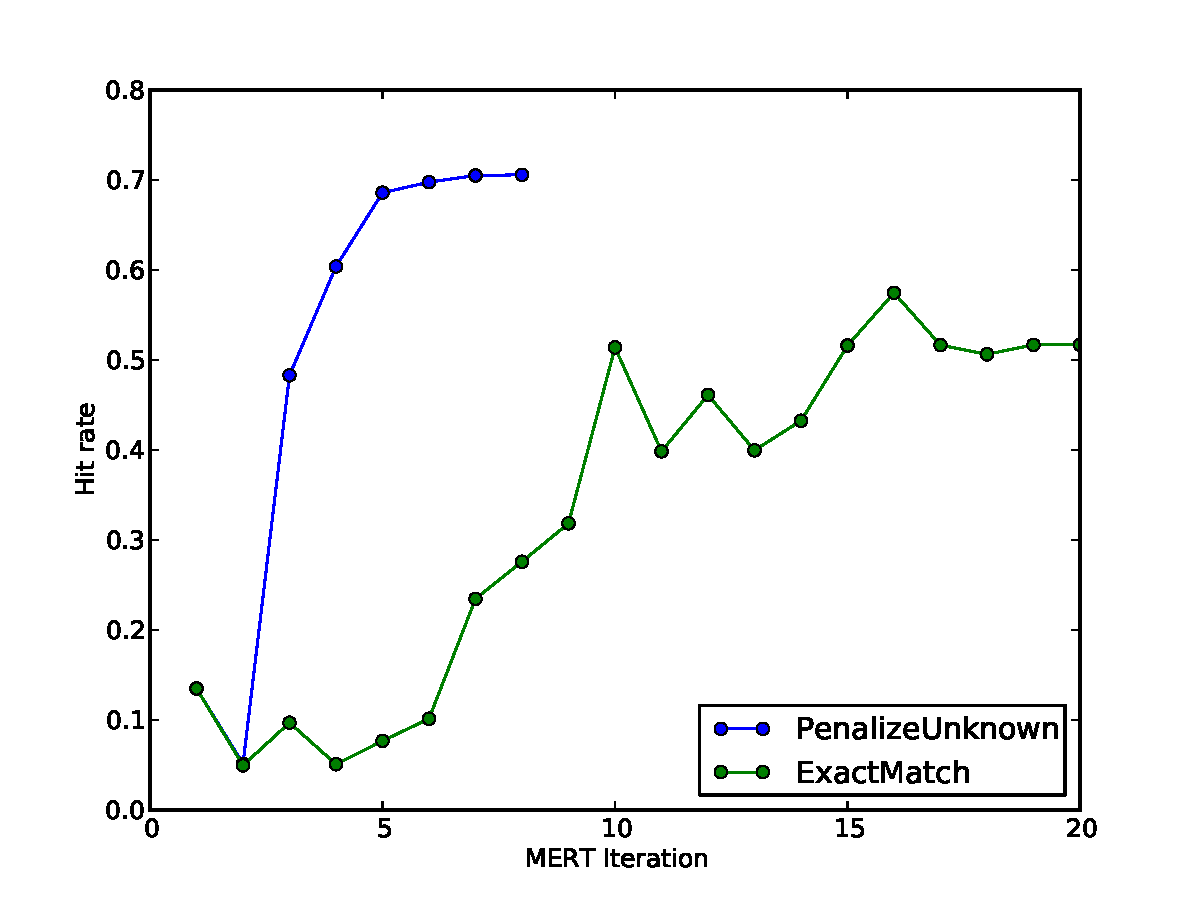
\includegraphics[width=12cm]{img/hit-rates-plot.pdf}
    \end{center}

    \caption[]{
}

    \label{hit:rates:plot}
\end{figure}


To see the differences between \metric{ExactMatch} and \metric{PenalizeUnknown},
we have plotted the values of hit rates computed in each MERT iteration in the figure
\ref{hit:rates:plot}.



